\section{The Algebraic Defect Framework}\label{sec:defect}

The failure of geometric compression reveals a fundamental constraint: any
method that \emph{moves} symbols between vertices risks violating the
injectivity requirement of the arrangement graph. The algebraic defect framework
circumvents this trap entirely by abandoning vertex-level transformations in
favor of \emph{coordinate-level counting}. Rather than asking ``can we shift
vertex $v$ to reduce the boundary?'' we ask ``how many distinct projections
(roots) does $V'$ cast along each coordinate?'' This root-counting perspective
is immune to the injectivity constraint because it never attempts to reassign
symbols---it merely observes the fiber structure that the set $V'$ already
induces.

Concretely, we count global algebraic roots. The sum $U(V')$ represents the
total number of 1-dimensional ``fibers'' (coordinate-aligned cliques) that
intersect our set $V'$. Each root $r$ acts as a fixed backbone that our set
projects onto along a specific dimension.

The framework utilizes a double-counting correction. By counting the available
alphabet symbols, every unique root $r \in U_p(V')$ can be extended to exactly
$(n - k + 1)$ valid vertices in the graph. Subtracting the internal fibers
mapping into $V'$ yields the strictly external coordinate edges
$E_{\mathrm{cand}}$:
\begin{align}\label{eq:ecand}
	E_{\mathrm{cand}} & = \sum_{p=1}^k \Big( |U_p(V')| \cdot (n - k + 1) \Big) - |V'| \cdot k \nonumber                           \\
	                  & = \left(\sum_{p=1}^k |U_p(V')|\right)(n-k) - \left(|V'| \cdot k - \sum_{p=1}^k |U_p(V')|\right) \nonumber \\
	                  & = U(V') \cdot (n-k) - D(V').
\end{align}

Because external neighbors may be hit by multiple dimensions, we subtract the
\emph{Cross-Collisions} $X(V')$ to retrieve the exact boundary of unique
vertices. We formally define $X(V')$ as the sum of over-counted boundary
adjacencies:
\begin{equation}\label{eq:cross-collision}
	X(V') = \sum_{v \in \extbd(V')} (\text{deg}_{V'}(v) - 1).
\end{equation}

The exact boundary size is then:
\begin{equation}\label{eq:boundary}
	\left| \extbd(V') \right| = U(V') \cdot (n - k) - \big(X(V') + D(V')\big).
\end{equation}
The algebraic engine of this framework relies on a fundamental subadditivity
inequality for $\Eseq(\cdot)$ (Definition~2.5). While this inequality reflects
the classical inductive step in Harper's edge-isoperimetric theorem for Boolean
hypercubes \cite{harper1966optimal}, we formally mechanize it here to bound
arbitrary fiber partitions in $A(n,k)$.

\begin{lemma}[Subadditivity of A000788]\label{lem:subadditivity}
	For all $x, y \in \mathbb{N}$:
	\begin{equation}\label{eq:subadditivity}
		\Eseq(x) + \Eseq(y) + \min(x, y) \leq \Eseq(x + y).
	\end{equation}
\end{lemma}

\begin{proof}
By strong induction on $x + y$: assume \eqref{eq:subadditivity} holds for all
pairs summing to less than $x + y$. Case-split on the parity of both $x$ and $y$
(four cases) and expand via the even/odd recurrences $\Eseq(2m) = 2\, \Eseq(m) +
m$ and $\Eseq(2m+1) = \Eseq(m) + \Eseq(m+1) + m$. In each case, the recurrences
halve the arguments, reducing the inequality to the inductive hypothesis at a
strictly smaller sum. Mechanically verified in Lean~4
(\texttt{E\_add\_min\_le}).
\end{proof}

For fiber sizes $c_1,\ldots,c_m$, write $y=|U_p(V')|$. The coordinate projection
is injective on each fiber, whose roots form a subset of $U_p(V')$, so $\max_i
c_i\le y$; iterating Lemma~\ref{lem:subadditivity} while tracking this maximum
yields $\sum_i \Eseq(c_i)+R-y\le\Eseq(R)$, the multi-way bound used below.
Consequently, the Hamming Ball maximizes the defect among all connected
subgraphs.

\begin{theorem}[Defect Bound]\label{thm:defect}
	For any $R$-element subset $V' \subseteq V(A(n,k))$:
	\begin{equation}\label{eq:defect-bound}
		D(V') \leq \Eseq(R).
	\end{equation}
	Equivalently, $U(V') \geq R \cdot k - \Eseq(R)$.
\end{theorem}

\begin{proof}
By strong induction on $R$. For $R \ge 2$, choose a coordinate $p$ at which two
vertices of $V'$ disagree and partition $V'$ into fibers $\{F_\alpha\}$ by the
symbol $\alpha$ at position $p$. Each fiber is strictly smaller than $V'$, so
the inductive hypothesis gives $D(F_\alpha) \leq \Eseq(|F_\alpha|)$. The
root-disjointness structure at coordinates $q \neq p$ yields the decomposition
$D(V') \leq \sum_\alpha D(F_\alpha) + R - y$, where $y = |U_p(V')|$. Applying
the generalized partition subadditivity (iterated Lemma~\ref{lem:subadditivity})
closes the induction. Mechanically verified in Lean~4
(\texttt{sum\_unique\_roots\_lower\_bound}).
\end{proof}

Instead of relying on a dimension-independent bound on the combined waste (which
is sensitive to $n-k$ for sub-optimal topologies), the global boundary
minimality is captured by the following universal boundary inequality. Together
with the evaluation of the Hamming Ball, these two propositions form our
extremal framework.

\begin{proposition}[Universal Boundary Inequality]\label{prop:universal}
	For every $R$-element subset $V' \subseteq V(A(n,k))$:
	\begin{equation}\label{eq:universal-bound}
		\left|\extbd(V')\right| \ge \big(R \cdot k - \Eseq(R)\big) \cdot (n - k) - \Cconst(R).
	\end{equation}
\end{proposition}

\begin{proposition}[Hamming Ball Evaluation]\label{prop:hb-eval}
	The lexicographic Hamming Ball $\mathrm{HB}_R$ achieves equality:
	\begin{equation}\label{eq:hb-eval}
		X(\mathrm{HB}_R) + \Eseq(R) = \Cconst(R).
	\end{equation}
\end{proposition}

\begin{remark}
These propositions encode the extremal content of a vertex-isoperimetric
compression theorem applied to the arrangement graph fiber structure: Harper's
edge-isoperimetric theorem \cite{harper1966optimal} for the binary ($n=2$)
case, and the more general Bollob\'{a}s--Leader compression theorem for
vertex-isoperimetric inequalities on $n$-ary Hamming graphs
\cite{bollobas1991vertex} for $n > 2$. The Kruskal-Katona shadow theorem
\cite{kruskal1963number,katona1968theorem} is a related but distinct result
about uniform set systems (binary layers of the hypercube); it is not by
itself sufficient for the $n$-ary transfer required here (see the discussion
of this citation issue in the proof-sketch notes accompanying this project).
Proposition~\ref{prop:hb-eval} is
computationally verified through $R \le 160$ by constructing $\mathrm{HB}_R$ and
enumerating its boundary in $A(2R, R)$ (Appendix~\ref{app:engine}).
Proposition~\ref{prop:universal} is tested exhaustively over connected
$R$-vertex subsets for $R \le 10$ by enumerating every non-isomorphic connected
$R$-vertex subgraph via the \texttt{nauty}-based engine (Section~3), and
separately over \emph{all} (including disconnected) $R$-vertex subsets, for
$R \le 6$ across 26 parameter rows of $A(n,k)$ (up to $3.24\times10^9$ subsets
in a single row), with no counterexample found in either search. Because
both searches are bounded in $R$, this remains only partial computational
evidence; the proposition is
open, not yet proven, for general $R$. Conceptually,
Section~\ref{sec:sandwich}'s asymptotic-dominance argument explains why, once
$n-k$ is large relative to the fixed cluster size $R$, no sub-optimal topology's
savings in cross-collisions can outweigh its linear-in-$(n-k)$ penalty for
missing defect --- an argument that holds regardless of $R$, but which by itself
does not establish the exact universal bound at every finite scale; that
stronger, exact statement is exactly the content of
Proposition~\ref{prop:universal} above. A further gap, independent of these two
propositions, is the \emph{boundary-to-extraconnectivity reduction}: even with
an exact minimum-boundary theorem, one must still show that (i)~deleting the
Hamming ball's external boundary leaves every remaining component with at least
$R$~vertices, and (ii)~every minimum $(R{-}1)$-extra cut can be reduced to
isolating one connected component of exactly $R$~vertices---minimizing over
connected $R$-sets whose boundary deletion is itself a valid $(R{-}1)$-extra
cut---without increasing the cut. This reduction is not addressed in the Lean
formalization, whose capstone proves only a statement about external-neighbor
sets of $R$-element subsets. In the Lean 4 formalization, rather than declaring
these propositions as global axioms, we express this dependency by
parameterizing the public capstone theorem with the explicit
\texttt{UniversalLowerBound} hypothesis. The Hamming-ball collision evaluation
is supplied by the direct Lean proof. This cleanly isolates the classical
extremal set theory from the novel algebraic machinery
while ensuring that the compiled theorems are completely transparent, verified,
and free of raw, uninstantiated axiom commands.
\end{remark}

Combining these propositions with the boundary decomposition yields our main
result:

\begin{theorem}[Conditional Minimum-Boundary Theorem]\label{thm:main}
\textup{(Conditional on Propositions~\ref{prop:universal}
and~\ref{prop:hb-eval}; see the remark following them for their verification
status.)} For all $R \ge 2$ and $n \ge k \ge 1$:
	\begin{enumerate}
\item[\textup{(i)}] \textbf{Universal lower bound.} Every $R$-element subset $V'
\subseteq V(A(n,k))$ satisfies
		      \begin{equation}\label{eq:lower-bound}
			      \left|\extbd(V')\right| \ge \big(R \cdot k - \Eseq(R)\big) \cdot (n - k) - \Cconst(R).
		      \end{equation}
\item[\textup{(ii)}] \textbf{Achievability.} When $n - k \ge \lceil \log_2 R
\rceil$ and $k \ge \lceil \log_2 R \rceil$, the lexicographic Hamming Ball
$\mathrm{HB}_R$ achieves this bound with equality:
		      \begin{equation}\label{eq:hb-boundary}
			      \left|\extbd(\mathrm{HB}_R)\right| = \big(R \cdot k - \Eseq(R)\big) \cdot (n - k) - \Cconst(R)
		      \end{equation}
where $\Eseq(R)$ and $\Cconst(R)$ are as in Definition~2.5. Writing $d = \lceil
\log_2 R \rceil$, the correction constant admits the closed form
		      \begin{equation}\label{eq:cconst}
			      \Cconst(R) = R(d + 1) - 2^d - \Eseq(R).
		      \end{equation}
	\end{enumerate}
The embedding condition in (ii) ensures the graph is large enough to fit a
$d$-dimensional hypercube.
\end{theorem}

\begin{corollary}[Conditional Extraconnectivity Formula]\label{cor:extraconnectivity}
\textup{(Conditional on Theorem~\ref{thm:main} and the
boundary-to-extraconnectivity reduction described in the remark following
Propositions~\ref{prop:universal}--\ref{prop:hb-eval}.)} When $n - k \ge \lceil
\log_2 R \rceil$ and $k \ge \lceil \log_2 R \rceil$,
	\begin{equation}\label{eq:extraconnectivity}
		\kappa_{R-1}(A(n,k)) = \big(R \cdot k - \Eseq(R)\big) \cdot (n - k) - \Cconst(R).
	\end{equation}
\end{corollary}

\begin{remark}[Closed-form evaluation of $\Cconst$]
The summation $\sum_{i=1}^{R-1} \lceil \log_2(i+1) \rceil$ admits a closed form
by grouping indices by dimension level. For each $j \ge 1$, exactly $2^{j-1}$
indices satisfy $\lceil \log_2(i+1) \rceil = j$ (those with $2^{j-1} < i+1 \le
2^j$). Summing the complete levels $j = 1, \ldots, d-1$ via the identity
$\sum_{j=1}^{m} j \cdot 2^{j-1} = (m-1) 2^m + 1$ and adding the partial level at
$j = d$ yields
	\begin{equation}\label{eq:ceillog-sum}
		\sum_{i=1}^{R-1} \lceil \log_2(i+1) \rceil = R\,\lceil \log_2 R \rceil - 2^{\lceil \log_2 R \rceil} + 1,
	\end{equation}
	eliminating the last summation from the formula for $\Cconst(R)$.
\end{remark}

\begin{proof}
\textbf{Part~(i).} The lower bound is established directly by
Proposition~\ref{prop:universal}.

\textbf{Part~(ii).} Proposition~\ref{prop:hb-eval} shows $X(\mathrm{HB}_R) +
\Eseq(R) = \Cconst(R)$. Substituting this into the boundary decomposition
equation~\eqref{eq:boundary} for $\mathrm{HB}_R$, where $U(\mathrm{HB}_R) = R
\cdot k - \Eseq(R)$, yields
	\begin{equation}
		\left|\extbd(\mathrm{HB}_R)\right| = \big(R \cdot k - \Eseq(R)\big) \cdot (n - k) - \Cconst(R),
	\end{equation}
meaning the lexicographic Hamming Ball achieves the universal lower bound with
equality. The embedding condition ensures $A(n,k)$ has a large enough alphabet
and enough positions to realize $\mathrm{HB}_R$ as an induced subgraph.
\end{proof}

\begin{corollary}[System-Level Diagnosability]\label{cor:diagnosis}
Under the PMC and MM* models, the $g$-extra diagnosability $t_g(G)$ is derived
from the $g$-extra connectivity via $t_g(G) = \kappa_g(G) + g + 1$ when $|V(G)|
\ge 2g + 3$ \cite{cheng2023augmented}. Conditional on Theorem~\ref{thm:main},
the additional reduction from minimum $R$-set boundary to
$(R{-}1)$-extraconnectivity, and the standard size hypotheses of the relevant
PMC/MM* diagnosis theorem, the exact $(R{-}1)$-extra diagnosability of the
arrangement graph follows, extending recent diagnostic advances (e.g., adaptive
local diagnosis \cite{zhang2026three}) to arbitrary fault boundaries.
\end{corollary}

\begin{figure}[H]
	\centering
	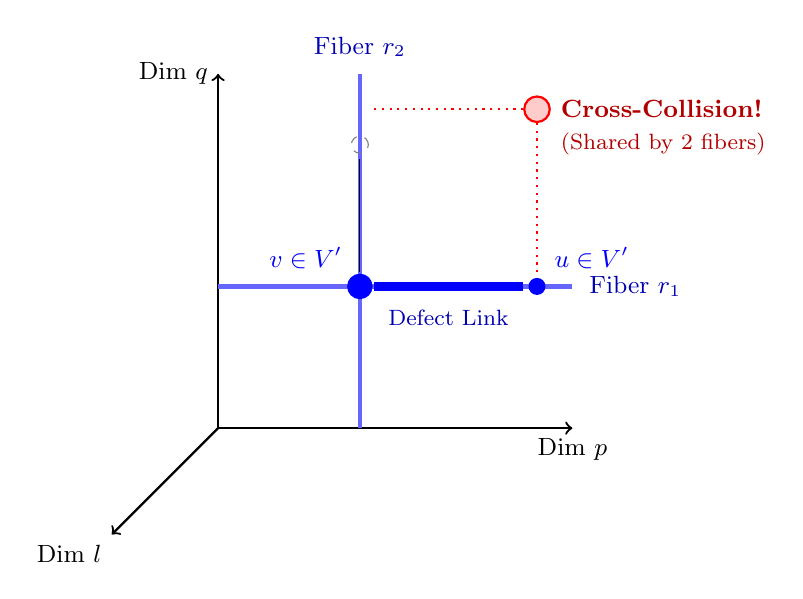
\begin{tikzpicture}[scale=0.9, font=\small]
		% Draw 3D-like axes
		\draw[->, thick] (0,0) -- (5,0) node[anchor=north] {Dim $p$};
		\draw[->, thick] (0,0) -- (0,5) node[anchor=east] {Dim $q$};
		\draw[->, thick] (0,0) -- (-1.5,-1.5) node[anchor=north east] {Dim $l$};

		% Draw "Fibers" as lines
		\draw[blue!60, ultra thick] (0,2) -- (5,2);
		\node[blue!70!black, anchor=west] at (5.1,2) {Fiber $r_1$};

		\draw[blue!60, ultra thick] (2,0) -- (2,5);
		\node[blue!70!black, anchor=south] at (2,5.1) {Fiber $r_2$};

		% Draw set V' as circles on the fibers
		\fill[blue] (2,2) circle (0.18) node[above left=0.1cm] {$v \in V'$};
		\fill[blue] (4.5,2) circle (0.12) node[above right=0.1cm] {$u \in V'$};

		% Draw internal edges (Defect)
		\draw[blue, line width=3.5pt] (2.2,2) -- (4.3,2);
		\node[blue!70!black, font=\footnotesize, anchor=north] at (3.25,1.8) {Defect Link};

		% Draw boundary vertices
		\draw[gray, dashed] (2,4) circle (0.12) node[left=0.1cm] {$\extbd$};
		\draw (2,2.2) -- (2,3.8);

		% Draw Cross-Collision
		\fill[red!20, draw=red, thick] (4.5,4.5) circle (0.18);
		\node[red!70!black, anchor=west] at (4.7,4.5) {\textbf{Cross-Collision!}};
		\node[red!70!black, font=\footnotesize, anchor=north west] at (4.7,4.3) {(Shared by 2 fibers)};

		\draw[red, dotted, thick] (2.2,4.5) -- (4.3,4.5);
		\draw[red, dotted, thick] (4.5,2.2) -- (4.5,4.3);
	\end{tikzpicture}
	\caption{The boundary decomposition
	$|\extbd(V')| = U(V') \cdot (n-k) - (X(V') + D(V'))$: defect links $D$
	shield internal vertices, while cross-collisions $X$ correct for boundary
	overlaps across coordinates.}
	\label{fig:structure}
\end{figure}

\begin{figure}[H]
	\centering
	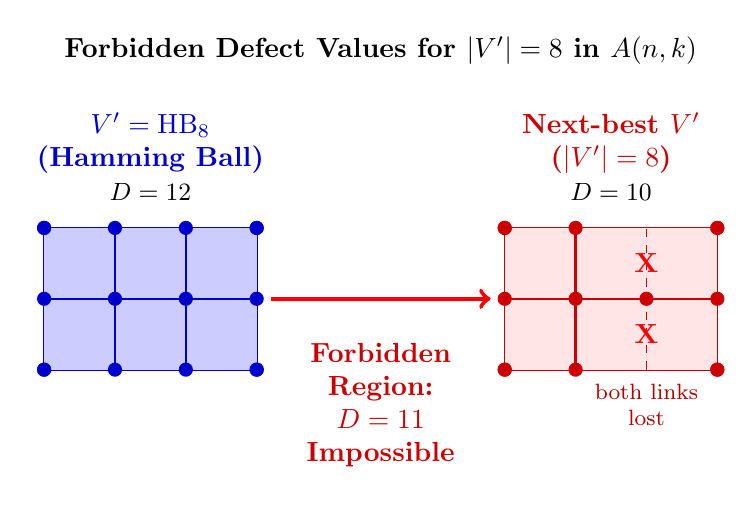
\begin{tikzpicture}[scale=0.9, font=\small]
		% Title
		\node[font=\bfseries] at (4.75, 5.5) {Forbidden Defect Values for $|V'|=8$ in $A(n,k)$};

		% Left side: Optimal subset (Hamming Ball)
		\node[align=center, font=\bfseries, text=blue!80!black] at (1.5, 4.2) {$V'=\mathrm{HB}_8$ \\ (Hamming Ball)};
		\node at (1.5, 3.5) {$D = 12$};

		\draw[thick, blue!80!black] (0,1) rectangle (3,3);
		\fill[blue!20] (0,1) rectangle (3,3);
		\foreach \x in {0,1,2,3} \foreach \y in {1,3} \fill[blue!80!black] (\x,\y) circle (0.1);
		\foreach \y in {1,2,3} \foreach \x in {0,3} \fill[blue!80!black] (\x,\y) circle (0.1);
		\draw[blue!80!black, thick] (0,2) -- (3,2);
		\draw[blue!80!black, thick] (1,1) -- (1,3);
		\draw[blue!80!black, thick] (2,1) -- (2,3);
		\fill[blue!80!black] (1,2) circle (0.1);
		\fill[blue!80!black] (2,2) circle (0.1);

		% Right side: Second Best subset
		\begin{scope}[xshift=1.5cm]
			\node[align=center, font=\bfseries, text=red!80!black] at (6.5, 4.2) {Next-best $V'$ \\ ($|V'|=8$)};
			\node at (6.5, 3.5) {$D = 10$};

			\draw[thick, red!80!black] (5,1) rectangle (8,3);
			\fill[red!10] (5,1) rectangle (8,3);
			\foreach \x in {5,6,8} \foreach \y in {1,3} \fill[red!80!black] (\x,\y) circle (0.1);
			\foreach \y in {1,2,3} \foreach \x in {5,8} \fill[red!80!black] (\x,\y) circle (0.1);
			\draw[red!80!black, thick] (5,2) -- (8,2);
			\draw[red!80!black, thick] (6,1) -- (6,3);
			\fill[red!80!black] (6,2) circle (0.1);
			\fill[red!80!black] (7,2) circle (0.1);
			\draw[red!80!black, dashed] (7,1) -- (7,3);
			\node[text=red, font=\bfseries] at (7, 2.5) {X};
			\node[text=red, font=\bfseries] at (7, 1.5) {X};
			\node[text=red!70!black, font=\footnotesize, align=center] at (7, 0.5) {both links\\lost};
		\end{scope}

		% Connecting arrow with gap label
		\draw[->, ultra thick, red] (3.2, 2) -- (6.3, 2);
		\node[align=center, font=\bfseries, text=red!80!black] at (4.75, 0.5) {Forbidden\\Region:\\$D=11$\\Impossible};
	\end{tikzpicture}
	\caption{The fracture gap at $R=8$: $\mathrm{HB}_8$ achieves $D=12$. In
	$A(n,k)$, defect links arise from root-sharing---two vertices that agree
	on all coordinates but one. Each link therefore has a ``twin'' at the same
	coordinate, so removing one vertex from a root pair destroys both links
	simultaneously. This makes $D=11$ impossible; the next achievable value is
	$D=10$.}
	\label{fig:fracture}
\end{figure}
